\documentclass[pdftex,12pt,a4paper]{article}
\usepackage{bachelorarbeit}
\usepackage{subfigure}
\usepackage[square]{natbib}
\usepackage[center]{caption}
\usepackage[english]{babel}

% Zum Setzen von URLs
\usepackage{color}
\definecolor{darkred}{rgb}{.25,0,0}
\definecolor{darkgreen}{rgb}{0,.2,0}
\definecolor{darkmagenta}{rgb}{.2,0,.2}
\definecolor{darkcyan}{rgb}{0,.15,.15}
\usepackage[plainpages=false,bookmarks=true,bookmarksopen=true,colorlinks=true,
  linkcolor=darkred,citecolor=darkgreen,filecolor=darkmagenta,
  menucolor=darkred,urlcolor=darkcyan]{hyperref}

% Hier die eigenen Daten eintragen
\global\arbeit{Bachelorarbeit}
\global\titel{Specification of a kernel}
\global\bearbeiter{Andrea Kuchar}
\global\betreuer{Dr Martin Hofmann, Ulrich Sch\"opp}
\global\abgabetermin{03-30-2018}
\global\ort{Munich}
\global\fach{Computer Science}

\begin{document}
	
	% Cover
	\deckblatt
	
	% Declaration of authorship
	\erklaerung
	
	% Abstract
	\clearpage
	\pagenumbering{none}
	\selectlanguage{english}
	\section*{Abstract}
	
	 The thesis investigates the question if the specification of the seL4 access control system is strong enough to imply the Noninterference property. 
Using the verification of the Take-Grant-Protection Model \citep{TakeG} I deduce from it the Unwinding Theorem conditions of the nondeterministic intransitive Noninterference Model \citep{NonOp}. 
As the specifications and proofs of the take-grant model is developed in the theorem proof assistant Isabelle/HOL I use the same to verify the implication. 
	

	\newpage
	
	% tableofcontents
	\tableofcontents
	\pagenumbering{Roman}
	
	\clearpage
	% Hier beginnt der eigentliche Text
	\section{Introduction}
	\pagenumbering{arabic}
	SeL4 is a high-assurance, high-performance microkernel, primarily developed, maintained and formally verified by NICTA (now Trustworthy Systems Group at Data61) for secure embedded systems.
In this thesis, the access control specification in terms of a classical take-grant model is proven to be sound enough to deduce from it the Noninterference property.
The classical security property of noninterference assures that there is no unwanted information flow within a system.
For the proof of information flow security  \citep{NonOp} a variant of intransitive noninterference was applied.
D. Elkaduwe, G. Klein and K. Elphinstone present in their paper \citep{TakeG} an abstract specification of the seL4 access control system in the context of a classical take-grant model and a formal proof of its decidability. With this, they showed how confined subsystems can be enforced.
The presented security proofs are not yet connected with the actual kernel implementation.
For the named noninterference property the authors \citep{NonOp} showed that it is preserved by refinement. So the goal of this thesis is the implication of the noninterference property from the take-grant specification. With this implication it is possible to create a connection with the actual kernel implementation.
All proofs and specifications in this thesis are developed in the theorem proof assistant Isabelle/HOL

	
	\clearpage
	
	\section{Requirements}
	\subsection{The seL4 Microkernel}
	The seL4 \citep{sel4} ist a small operation system kernel. It's based on the in the 1990s developed L4 microkerel and provieds a minimal number of services to applications, such as abstraction for virutal address spaces, threads, inter process comunication (IPC). 
	
	\subsubsection{System Calls}
	The kernel provied severel system calls: \\
	\begin{itemize}
	\item \texttt{send()}: The system call argument ist delivered to the target object and the application is allowed to continue. If the target is not able to receive and/or process the arguments immediately, the sending application will be blocked until the arguments can be delivered.
	\item \texttt{NBSend()}: Like \texttt{send()}. Exception: If the message is not deliverable it's silently droped.
	\item \texttt{Call()}: Like \texttt{send()} but the application is blocked until the object provieds a response, or the receiving application replies. \\
	If tthe argument is delivered to an application via Endpoint the receiver needs the right to respond to the sender. So in this case an additional capability is added to the arguments. 
	\item \texttt{Wait()}: If the target object is not ready \texttt{Wait()} is used by an application to block until the object is ready. 
	\item \texttt{Reply()}: Used to respond to a \texttt{Call()}, using the capability generated by the \texttt{Call()} operation.
	\item \texttt{ReplyWait()}: As a combination of \texttt{Reply()} and \texttt{Wait()} it's efficent for the common case that replying to a request and waiting for the next can be performed in a single system call. 
	\end{itemize}
	\newpage
	\subsubsection{Kernel Objects}
	The kernel objects can be invoked by applications. The following showes a brief overview of the kernel implemented objects. 
	\begin{itemize}
	\item \textbf{CNodes} \\
	Capabilities in seL4 are stored in kernel objects called \textbf{CNodes} with a fixed number of slots that can be empty or contain a capability. They have the following operations:
	\texttt{Mint()}, \texttt{Copy()}, \texttt{Move()}, \texttt{Mutate()}, \texttt{Rotate()}, \texttt{Delete()}, \texttt{Revoke()}, \texttt{SaveCaller()}, \texttt{Recycle()}
	\item \textbf{IPC Endpoints} \\
	For the \textit{interprocess communication} between threads the kernel supports synchronous (EP) and asynchronous (AsyncEP) endpoints. The capabilities to that endpoints can be limited as send-only or receive-only or be specified to pass capabilities through the endpoint.  
	\item \textbf{TCP} \\
	The \textit{thread control block} object represents a thread of execution in seL4. It needs a CSpace (provides the capabilities required to manipulate the kernel objects) and a VSpace (provides the virtual memory environment required to contain the code and data application). The connections are illustrated in Figure \ref{fig:intapp}. \\
	The TCB object has the following methods: \\
	\texttt{CopyRegisters(), ReadRegisters(), WriteRegisters(), SetPriority(), SetIPCBuffer(), SetSpace(), Configure(), Suspend(), Resume()}
	
	\begin{figure}[ht]
	\centering
		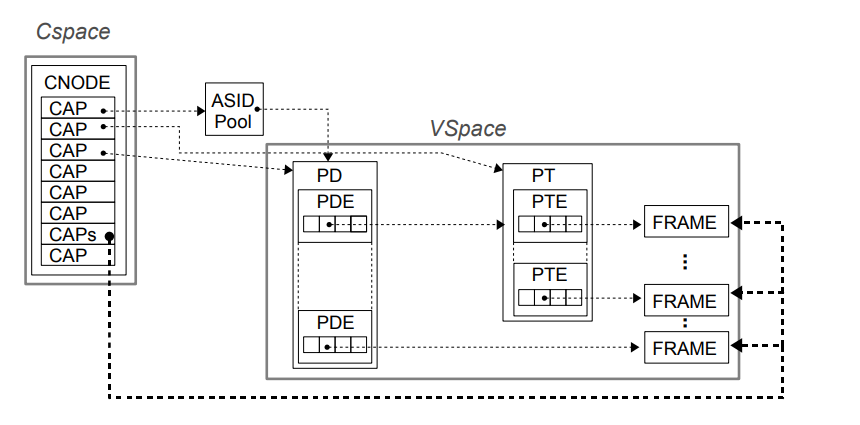
\includegraphics[width=0.8\textwidth]{./applicationIntern.png}
	\caption[Internal repersentation of application]{Internal representation of an application in seL4 \citep{sel4}}
	\label{fig:intapp}
	\end{figure}
	
	\item \textbf{Virtual Memory}\\
	A \textit{virtual address space} (VSpace) contains objects for managing virtual memory which largely directly correspond to those of the hardware: \\
	Page Directory, Page Table, Page, ASID Control, ASID Pool
	\item \textbf{Interrupt Objects} \\
	For device driver applications to be able to receive and acknowledge interrupts from hardware devices.
	\item \textbf{Untyped Memory} \\
	Untyped memory objects can be devieded into a group of smaller untyped memory objects. \texttt{Retype()} ist the only method untyped memory capabilities have. It creates a number of new kernel objects and returns capabilities to the new objects if it succeeds. 
	\end{itemize}
	
	\newpage
	\subsubsection{Memory Allocation Model}
	Important for the seL4 is that all kernel objects must be fully contributed for by capabilities. \\
	At boot time the kernel pre-allocates all the memory required for the kernel to run. This includes the space for kernel code, data and kernel stack. The ressource manager has full authority over the untyped memory (UM) objects, generated by deviding the remain memory into these objects. \\
	A capability to untyped memory can be refined into child capabilities, smaller sized untyped memory blocks or other kernel objects with the retype operation on UM objects. \\
	The creator of an kernel object has full authority over the object. This "full authority" depends on the the object type. \\
	Figure \ref{fig:systarch} shows a sample system architecture in wich a resource manager running at user-level  has the authority to the remaining untyped memory after boot strapping. 
	
	\begin{figure}[ht]
	\centering
		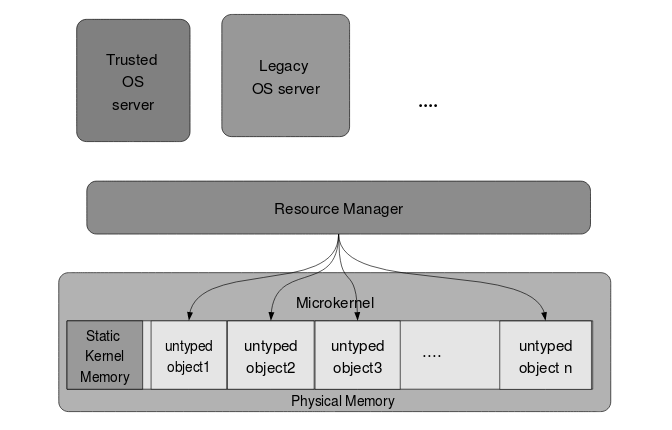
\includegraphics[width=0.8\textwidth]{./MemoryAllocation.png}
	\caption[Sample system architecture]{Sample System Configuration \citep{TakeG}}
	\label{fig:systarch}
	\end{figure}	
	
	\newpage
	\subsection{The Take-Grant Model}	
	
	
	\cleardoublepage
	\begin{thebibliography}{99}

	\bibitem{NonOp}
	T.\ Murray, D.\ Matichuk, M.\ Brassil, P.\ Gammie and G.\ Klein:	\\ 
	\href{http://www.ssrg.nicta.com/publications/nicta_full_text/6004.pdf}{%
		Noninterference for Operating System Kernels}. \\
    International Conference on Certified Programs and Proofs, pp. 126–142, Kyoto, Japan, December, 2012

	\bibitem{TakeG}
	D.\ Elkaduwe, G.\ Klein and K.\ Elphinstone:	\\ 
	\href{http://ts.data61.csiro.au/publications/nicta_full_text/1474.pdf}{%
		Verified Protection Model of the seL4 Microkernel}. \\
   	Technical Report NRL-1474, NICTA, October, 2007
   	
   	\bibitem{sel4}
	J.\ Andronick T.\ Bourke P.\ Derrin D.\ Greenaway D.\ Elkaduwe, G.\ Klein and K.\ Elphinstone R.\ Kolanski D.\ Matichuk T.\ Sewell S.\ Winwood:	\\ 
	\href{https://sel4.systems/Info/Docs/seL4-spec.pdf}{%
		Abstract Formal Specification of the seL4/ARMv6 API}. \\
   	Version 1.3

\end{thebibliography}
	
\end{document}